\section{Nota teórica}

\subsection{Características del Arduino UNO}
\subsubsection{Características generales}
EL Arduino UNO es un microcontrolador de baja potencia que contiene el ATMega328P @ \SI{16}{\mega\hertz} de tipo AVR de 8 bits con 131 instrucciones, cuya instrucciones son casi todos ejecutados en un ciclo de reloj. Adicionalmente, el microcontrolador cuenta con
\begin{itemize}
    \item 32 registros de 8 bits cada uno de propósito general,
    \item \SI{32}{\kilo\byte} de flash programable,
    \item \SI{1}{\kilo\byte} de EEPROM programable,
    \item \SI{2}{\kilo\byte} de SRAM,
    \item reloj en tiempo real (\it{real time counter}), 
    \item protección de memoria flash y EEPROM,
    \item tres contadores/temporizadores, dos de 8 bits y uno de 16 bits,
    \item seis canales de PWM,
    \item comparador analógico,
    \item seis convertidores analógico-digital por aproximación sucesiva de 10 bits cada uno,
    \item temporizador de \it{watchdog} programable,
    \item \it{serial peripheral interface} (SPI),
    \item \it{inter-integrated circuit} (I2C),
    \item \it{universal synchronous and asynchronous serial receiver and transmitter} (USART) \cite{datasheet, atmega}.
\end{itemize}
\subsubsection{Características eléctricas}
Los rangos absolutos que se deben respetar para este microcontrolador son
\begin{itemize}
    \item tensión operación máxima $V_\text{CC max}$: \SI{6}{\volt},
    \item tensión en el pin $\overline{\text{RESET}}$: \SI{-0.5}{\volt} a \SI{13}{\volt},
    \item tensión en los pines restantes: \SI{-0.5}{\volt} a $V_\text{CC} + \SI{0.5}{\volt}$,
    \item corriente máxima admitida en los pines de alimentación: \SI{200}{\milli\ampere},
    \item corriente máxima admitida para cada pin de I/O: \SI{40}{\milli\ampere},
    \item corriente máxima admitida para cada puerto: \SI{30}{\milli\ampere} \cite{datasheet, atmega}.

\end{itemize}

\subsubsection{Diagrama de bloques}
La figura \ref{mcu-diagram} ilustra el diagrama de bloques del microcontrolador ATMega328P. Algunos bloques de interés para este laboratorio son los bloques de conversión analógico-digital (A/D converter) para medición de tensión \& corriente, así como todos los bloques que conforman el procesador para ejecutar el programa como el \it{program counter}, el registro de instrucciones, el decodificador de instrucciones, la ALU y la memoria \cite{datasheet, atmega}. El resto de bloques del microcontrolador no serán utilizados para este proyecto.
\begin{figure}[H]
    \centering
    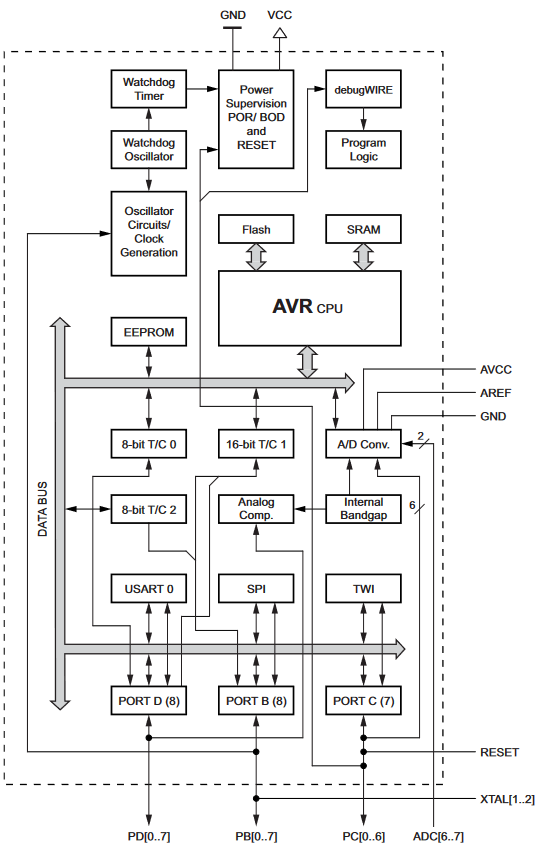
\includegraphics[width=14cm]{Imagenes/mcu-diagram.png}
    \caption{Diagrama de bloques del microcontrolador ATMega328P. Fuente y créditos: \cite{atmega}.}
    \label{mcu-diagram}
\end{figure}

\subsubsection{Diagrama de pines}
En la figura \ref{Fig: Diagrama_pines} se muestra el diagrama de pines del microcontrolador Arduino UNO \cite{datasheet}. Para el desarrollo de este proyecto se utilizaron los pines \tt{SCL} \& \tt{SDA} para conectar el Arduino UNO con la pantalla LCD, \tt{A0} \& \tt{A2} para medir la tensión y corriente, así como los pines de alimentación y tierra para suministrar potencia a la pantalla LCD y sensor de corriente.

\begin{figure}[H]
\centering
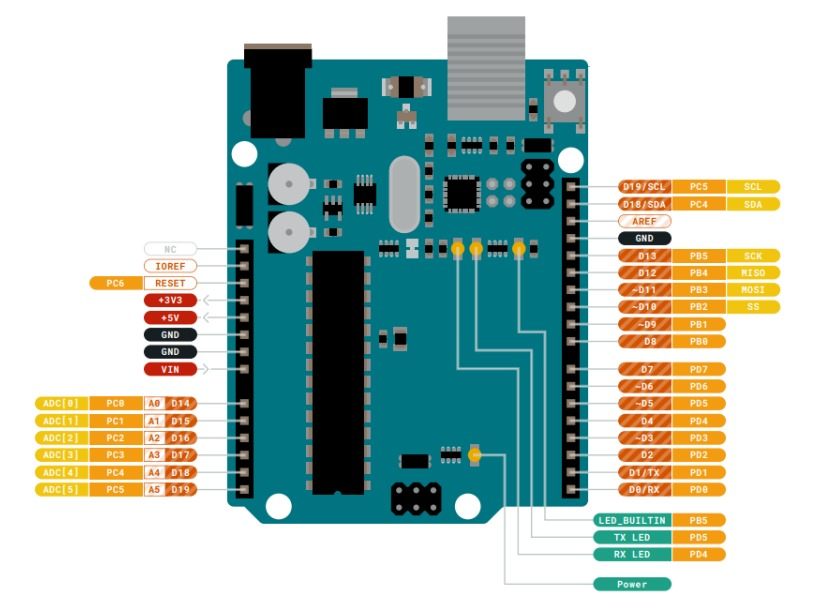
\includegraphics[width=\textwidth]{Imagenes/Diagrama_Pines.jpg} 
\caption{Diagrama de pines del Arduino UNO. Fuente y créditos: \cite{datasheet}.}
\label{Fig: Diagrama_pines}
\end{figure}